\documentclass{beamer}
\usetheme[pageofpages=of,% String used between the current page and the
                         % total page count.
          bullet=circle,% Use circles instead of squares for bullets.
          titleline=true,% Show a line below the frame title.
          alternativetitlepage=true,% Use the fancy title page.
       %   titlepagelogo=logo-polito,% Logo for the first page.
       %   watermark=watermark-polito,% Watermark used in every page.
       %   watermarkheight=100px,% Height of the watermark.
       %   watermarkheightmult=4,% The watermark image is 4 times bigger
                                % than watermarkheight.
          ]{Torino}

\setbeamertemplate{footline}{
  \begin{beamercolorbox}[wd=\paperwidth,ht=1ex,dp=1ex]{footline}
    \vspace{5pt} \hspace{1em} \insertframenumber/\inserttotalframenumber
  \end{beamercolorbox}
}

\author{Brendon J. Brewer}
\title{STATS 331 -- Introduction to Bayesian Statistics}
\institute{The University of Auckland}
\date{}


\linespread{1.3}
\usepackage{minted}
\usepackage[utf8]{inputenc}
\usepackage{dsfont}
\newcommand{\given}{\,|\,}

\begin{document}

\frame{\titlepage}

\begin{frame}
\begin{center}
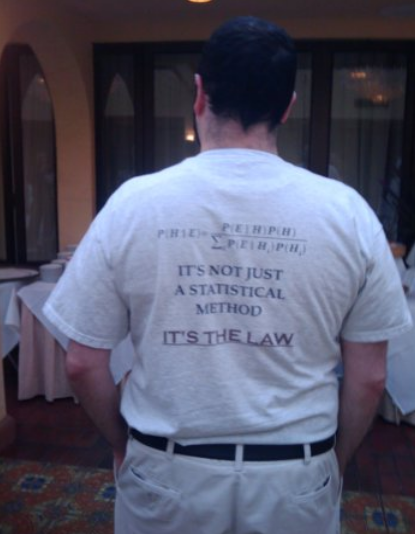
\includegraphics[width=0.4\textwidth]{images/tshirt.png} \\
Credit: lesswrong.com
\end{center}

\end{frame}

\begin{frame}
\begin{center}
\Large
Introduction to MCMC and the Metropolis Algorithm
\end{center}

\end{frame}

\begin{frame}
\frametitle{Philosphy}
\begin{itemize}
\item Markov Chain Monte Carlo (MCMC) algorithms are, strictly speaking, not
Bayesian.\pause
\item However, they are associated with Bayesian statistics because they happen
to be very useful in this area.\pause
\item They allow us to describe posterior distributions in more than one
dimension (more than one unknown parameter) quite easily.
\end{itemize}
\end{frame}

\begin{frame}
\frametitle{More Than One Parameter}
So far we have focused on single-parameter problems until we get used to the
Bayesian approach. But most real problems have more than one unknown parameter.
Imagine making a Bayes' Box:
\begin{center}
{\tiny
\begin{tabular}{|c|c|c|c|c|}
\hline
Parameter & Prior & Likelihood & Prior $\times$ Likelihood & Posterior \\
$(\theta_1, \theta_2)$  & $p(\theta_1, \theta_2)$ & $p(x \given \theta_1, \theta_2)$ & $p(\theta_1, \theta_2)p(x\given\theta_1, \theta_2)$ & $p(\theta_1, \theta_2\given x)$ \\
\hline
(0, 0) &  &  & & \\
(0, 0.1) &  &  & & \\
... & ... & ... & ... & ... \\
(0.1, 0) &  &  & & \\
(0.1, 0.1) & & & & \\
... & ... & ... & ... & ... \\
(1, 0.9) & & & & \\
(1, 1) & & & & \\
\hline
Total & 1 & & & 1 \\
\hline
\end{tabular}
} % tiny
\end{center}

\end{frame}

\begin{frame}
\frametitle{More Than One Parameter}
\begin{itemize}
\item Because each hypothesis is about the value of the {\em pair}
$(\theta_1, \theta_2)$, instead of say 100 grid points, we would need
100 $\times$~100. \pause
\item This is quite feasible, but annoying, because you would need 2D arrays
instead of vectors.\pause
\item However, in even higher dimensions (let's say 100) you would need
$10^{100}$ rows (or something like that) in your Bayes' Box.
That is not going to happen.
\end{itemize}


\end{frame}




\end{document}

